\documentclass[compress]{beamer}
\usepackage{irbookslide}
\usepackage{irilmenau2}
\usepackage{tikz}
\usepackage{url}
\usepackage{ifxetex}
%\RequireXeTeX
\usepackage{fontspec} % zahteva paket euenc
\usepackage{xunicode}
\usepackage{xltxtra}
\usepackage{polyglossia}
\usepackage{minted}
\usepackage{algorithmic}
\renewcommand{\algorithmicrequire}{\textbf{Input:}}
\renewcommand{\algorithmicensure}{\textbf{Output:}}
\usepackage{xcolor,colortbl}
\usepackage{textcomp}
%\setdefaultlanguage[script=Latin]{serbian}


\title{Stabla pretrage}
\author{\textcopyright \ \ Goodrich, Tamassia, Goldwasser}
\institute{Katedra za informatiku, Fakultet tehničkih nauka, Univerzitet u
Novom Sadu}
\date{2014.}
\subject{Predavanja sa ASP}

\begin{document}

\frame{\titlepage}

\section[Binarno]{Binarno stablo pretrage}
\begin{frame}[fragile]
  \frametitle{Mape sa poretkom}
  \begin{itemize}
    \item postoji relacija poretka nad ključevima 
    \item elementi se skladište prema vrednosti ključa
    \item pretrage ,,najbliži sused`` (nearest neighbor):
    \begin{itemize}
      \item nađi element sa najvećim ključem manjim ili jednakim $k$
      \item nađi element sa najmanjim ključem većim ili jednakim $k$
    \end{itemize}
  \end{itemize}
\end{frame}

\begin{frame}[fragile]
  \frametitle{Binarna pretraga}
  \begin{itemize}
    \item binarna pretraga može da pronađe ,,najbližeg suseda`` za mapu sa poretkom implementiranu pomoću niza koji je sortiran po ključu 
    \begin{itemize}
      \item u svakom koraku prepolovi se broj kandidata
      \item radi u $O(\log n)$ vremenu
    \end{itemize}
    \item primer: nađi 7 
  \end{itemize}
  \begin{center}
    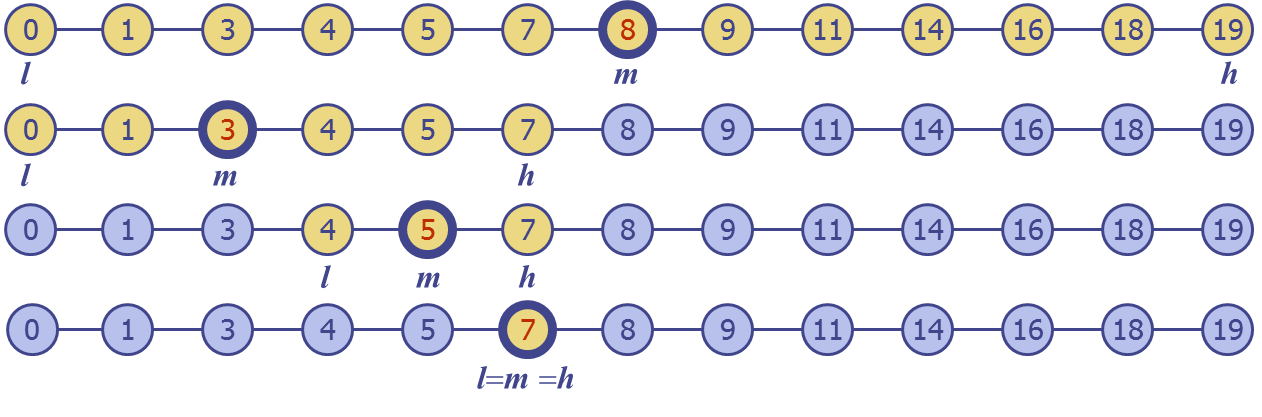
\includegraphics[width=10cm]{asp-11-pic01.png}
  \end{center}
\end{frame}

\begin{frame}[fragile]
  \frametitle{Tabela pretrage}
  \begin{itemize}
    \item tabela pretrage je mapa sa poretkom implementirana pomoću sortiranog niza 
    \begin{itemize}
      \item eksterni komparator za ključeve
    \end{itemize}
    \item performanse: 
    \begin{itemize}
      \item binarna pretraga je $O(\log n)$
      \item dodavanje je $O(n)$
      \item uklanjanje je $O(n)$
    \end{itemize}
    \item radi efikasno samo za mali broj elemenata ili tamo gde je pretraga česta a izmene retke (npr. provera kreditne kartice) 
  \end{itemize}
\end{frame}

\begin{frame}[fragile]
  \frametitle{Sortirana mapa ATP}
  \begin{itemize}
    \item standardne operacije mape 
  \end{itemize}
  \begin{center}
    \begin{tabular}{rp{8cm}}
      \textbf{\texttt{M[k]}} & vraća vrednost $v$ za ključ $k$ u mapi $M$; implementira je \texttt{\_\_getitem\_\_} \\ \hline
      \textbf{\texttt{M[k}=v} & dodaje novi element $(k, v)$ u $M$ ili menja postojeći; implementira je \texttt{\_\_setitem\_\_} \\ \hline
      \textbf{\texttt{del M[k]}} & uklanja element sa ključem $k$ iz $M$; implementira je \texttt{\_\_delitem\_\_} \\
    \end{tabular}
  \end{center}
  \begin{itemize}
    \item dodatne funkcionalnosti 
    \begin{itemize}
      \item sortiran redosled prilikom iteracije
      \item nađi veće: \myred{find\_gt}($k$)
      \item nađi u opsegu: \myred{find\_range}($start, stop$) 
    \end{itemize}
  \end{itemize}
\end{frame}

\begin{frame}[fragile]
  \frametitle{Binarno stablo pretrage}
  \begin{itemize}
    \item \myred{binarno stablo pretrage} je binarno stablo koje čuva $(k, v)$ parove u čvorovima $p$ tako da važi:
    \begin{itemize}
      \item ključevi koji se nalaze u \textbf{levom} podstablu od $p$ su \textbf{manji} od $k$
      \item ključevi koji se nalaze u \textbf{desnom} podstablu od $p$ su \textbf{veći} od $k$
    \end{itemize}
    %\item listovi ne čuvaju elemente
    \item inorder obilazak: ključevi u rastućem redosledu 
  \end{itemize}
  \begin{center}
    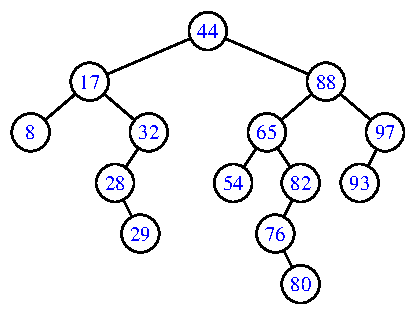
\includegraphics[width=6cm]{asp-11-pic02.pdf}
  \end{center}
\end{frame}

\begin{frame}[fragile]
  \frametitle{Pretraga u binarnom stablu}
  \begin{itemize}
    \item tražimo ključ $k$ polazeći od korena
    \item idemo levo ako je $k$ manji od tekućeg čvora
    \item idemo desno ako je $k$ veći od tekućeg čvora
    \item ako dođemo do lista, $k$ nije nađen
  \end{itemize}
  \begin{columns}
    \begin{column}[c]{6cm}
      \begin{center}
        Tražimo 65
        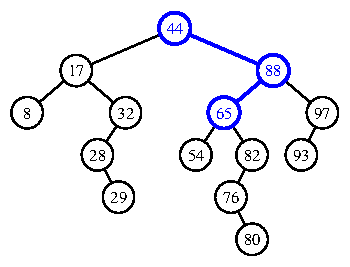
\includegraphics[width=6cm]{asp-11-pic03a.pdf}
      \end{center}
    \end{column}  
    \begin{column}[c]{6cm}
      \begin{center}
        Tražimo 68
        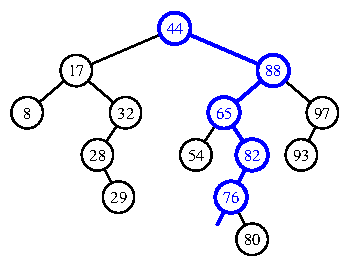
\includegraphics[width=6cm]{asp-11-pic03b.pdf}
      \end{center}
    \end{column}  
  \end{columns}
\end{frame}

\renewcommand{\algorithmiccomment}[1]{\hfill \{\myred{#1}\}}

\begin{frame}[fragile]
  \frametitle{Pretraga u binarnom stablu}
\myred{TreeSearch}($T, p, k$)
\begin{algorithmic}
\IF{$k = p.key$}
  \RETURN $p$ \COMMENT{pronađen}
\ELSIF{$k < p.key \land T.left(p) \neq None$}
  \RETURN TreeSearch($T, T.left(p), k$) \COMMENT{levo podstablo}
\ELSIF{$k > p.key \land T.right(p) \neq None$}
  \RETURN TreeSearch($T, T.right(p), k$) \COMMENT{desno podstablo}
\ENDIF
\RETURN None  \COMMENT{nije pronađen}
\end{algorithmic}
\end{frame}

\begin{frame}[fragile]
  \frametitle{Performanse pretrage u binarnom stablu}
  \begin{itemize}
    \item u svakom rekurzivnom pozivu spuštamo se za jedan nivo u stablu
    \item testiranje u okviru jednog nivoa je $O(1)$
    \item ukupan broj testova je $O(h)$, gde je $h$ visina stabla
  \end{itemize}
  \begin{center}
    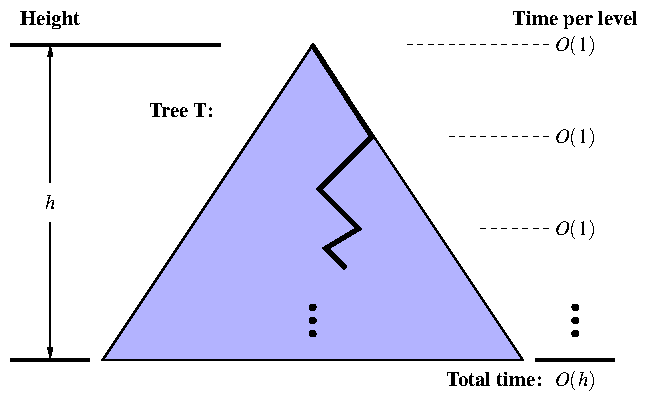
\includegraphics[width=8cm]{asp-11-pic04.pdf}
  \end{center}
\end{frame}

\begin{frame}[fragile]
  \frametitle{Dodavanje u stablo}
  \begin{itemize}
    \item dodajemo element $(k, v)$
    \item prvo tražimo $k$
    \item ako $k$ nije u stablu, došli smo do lista gde treba dodati čvor
    \item primer: dodajemo 68
  \end{itemize}
  \begin{columns}
    \begin{column}[c]{6cm}
      \begin{center}
        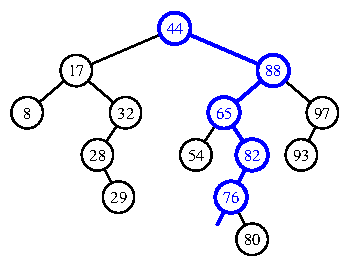
\includegraphics[width=6cm]{asp-11-pic05a.pdf}
      \end{center}
    \end{column}  
    \begin{column}[c]{6cm}
      \begin{center}
        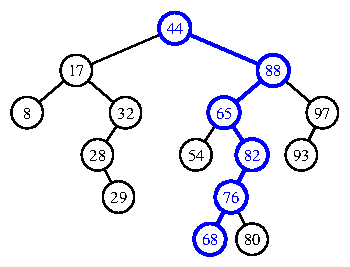
\includegraphics[width=6cm]{asp-11-pic05b.pdf}
      \end{center}
    \end{column}  
  \end{columns}
\end{frame}

\begin{frame}[fragile]
  \frametitle{Dodavanje u stablo}
\myred{TreeInsert}($T, k, v$)
\begin{algorithmic}
\STATE $p \leftarrow$ TreeSearch($T, T.root, k$)
\IF{$k = p.key$}
  \STATE $p.value \leftarrow v$  \COMMENT{ako već postoji zameni vrednost}
\ELSIF{$k < p.key$}
  \STATE $p$.add\_left($k, v$) \COMMENT{dodaj levo dete}
\ELSE
  \STATE $p$.add\_right($k, v$) \COMMENT{dodaj desno dete}
\ENDIF
\end{algorithmic}
  \begin{itemize}
    \item dodaje se uvek u list
  \end{itemize}
\end{frame}

\begin{frame}[fragile]
  \frametitle{Uklanjanje iz stabla}
  \begin{itemize}
    \item uklanjamo element sa ključem $k$
    \item prvo nađemo $k$
    \item ako $k$ ima najviše jedno dete
    \item primer: dodajemo 68
  \end{itemize}
  \begin{columns}
    \begin{column}[c]{6cm}
      \begin{center}
        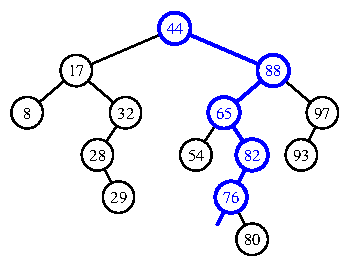
\includegraphics[width=6cm]{asp-11-pic05a.pdf}
      \end{center}
    \end{column}  
    \begin{column}[c]{6cm}
      \begin{center}
        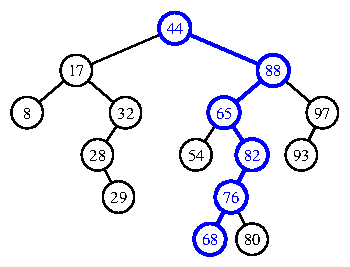
\includegraphics[width=6cm]{asp-11-pic05b.pdf}
      \end{center}
    \end{column}  
  \end{columns}
\end{frame}

\end{document}